\begin{figure}[ht!]
    \centering        
    \setlength{\tabcolsep}{2.0pt}      
    \begin{tabular}{ccccc} 
        \rotatebox{90}{\scriptsize\phantom{AA} No Encoder Pretrain} &                    
        
\includegraphics[width=0.19\textwidth]{figures/enc_pretrain/enc_pretrain_0_0.jpg} &
        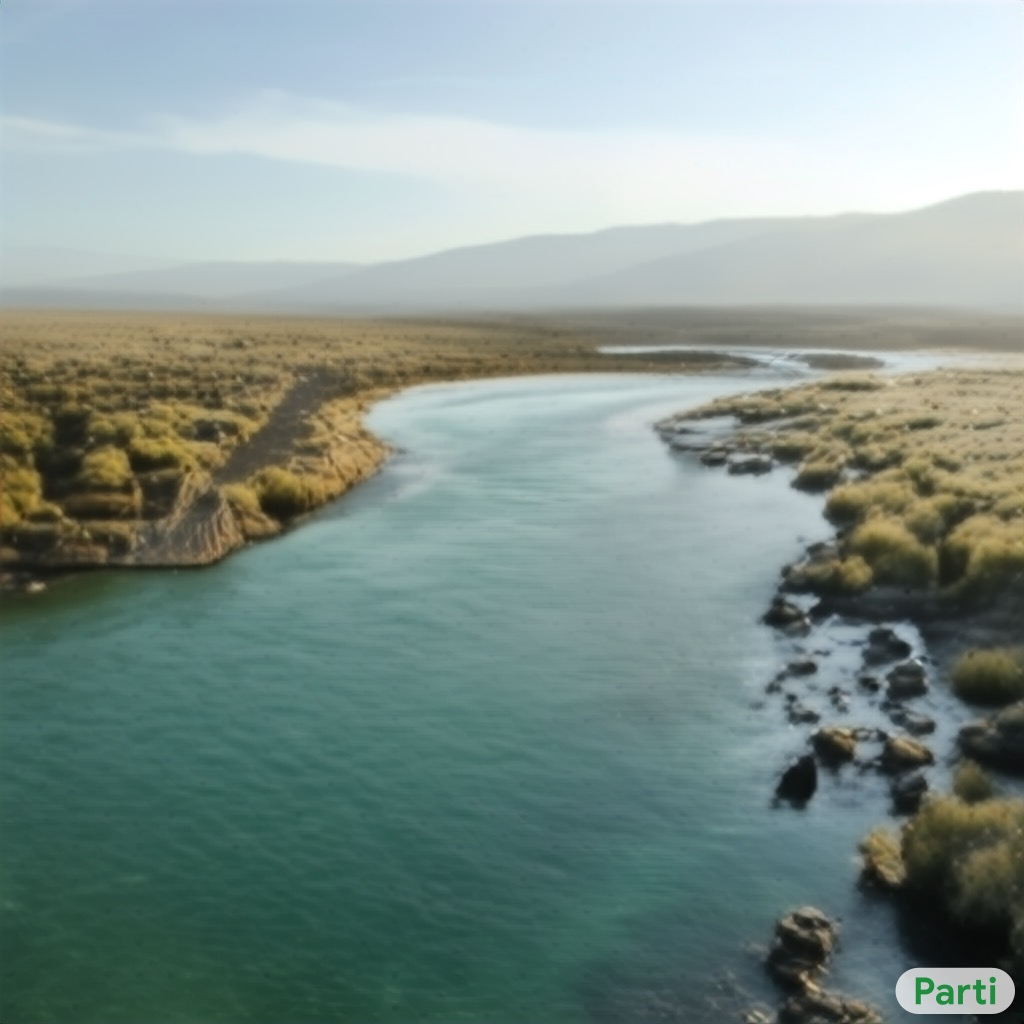
\includegraphics[width=0.19\textwidth]{figures/enc_pretrain/enc_pretrain_1_0.jpg} &
        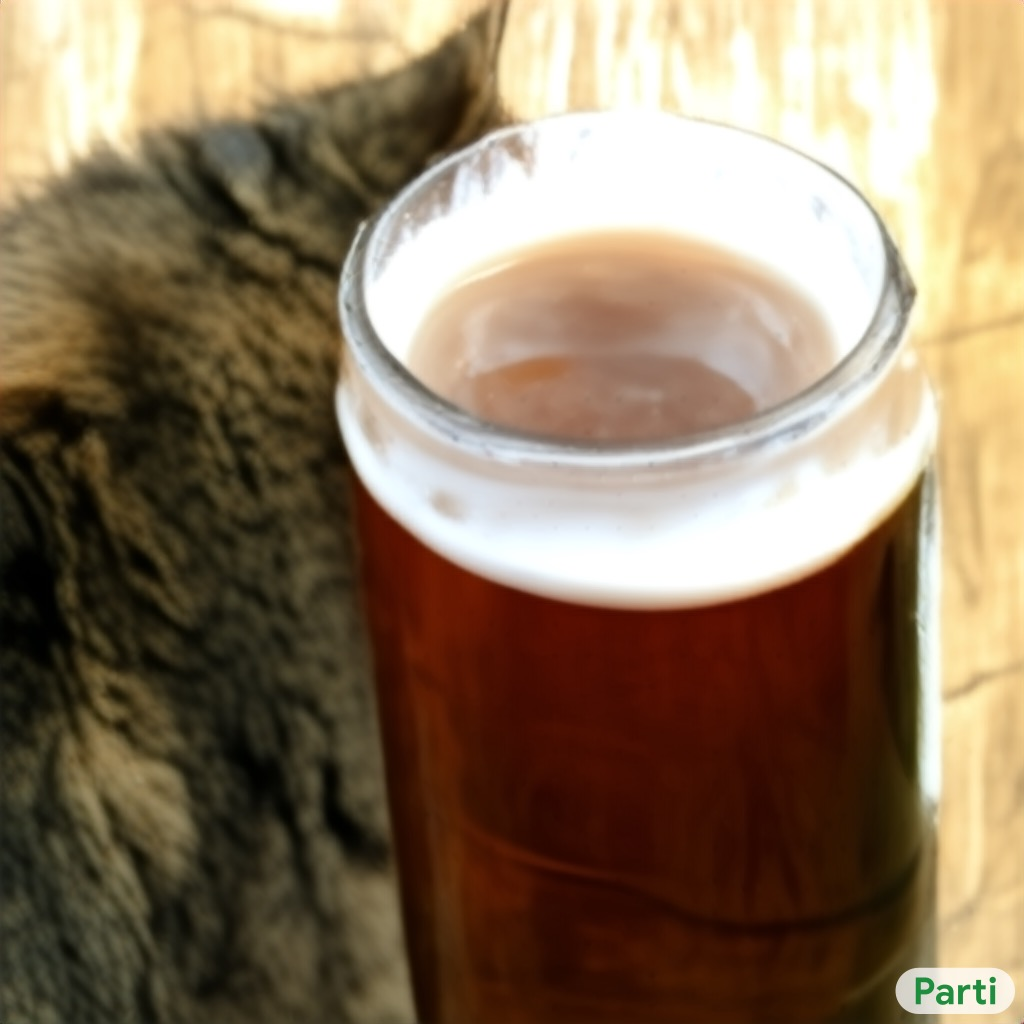
\includegraphics[width=0.19\textwidth]{figures/enc_pretrain/enc_pretrain_2_0.jpg} &
        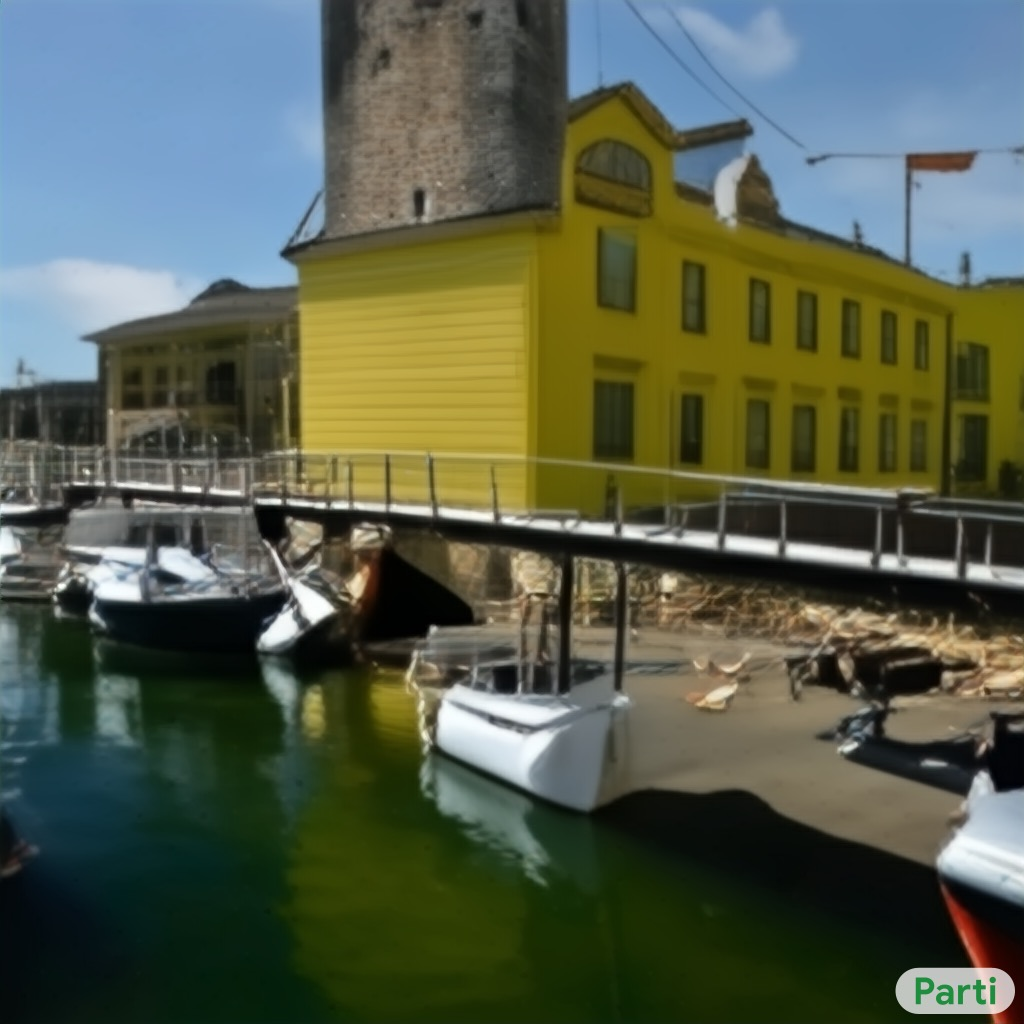
\includegraphics[width=0.19\textwidth]{figures/enc_pretrain/enc_pretrain_6_0.jpg} \\
                                                                                    
        \rotatebox{90}{\scriptsize\phantom{AA} Encoder Pretrain} &            
        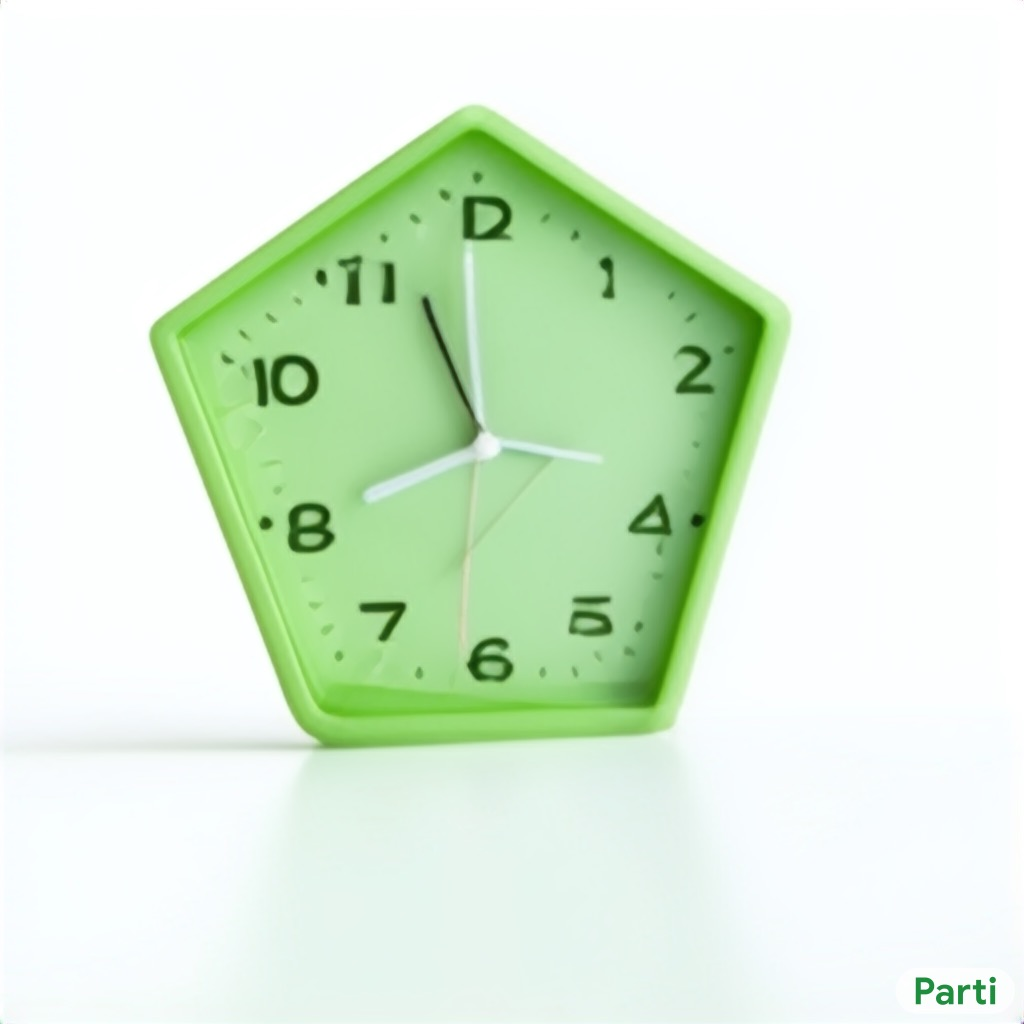
\includegraphics[width=0.19\textwidth]{figures/enc_pretrain/enc_pretrain_0_1.jpg} &
        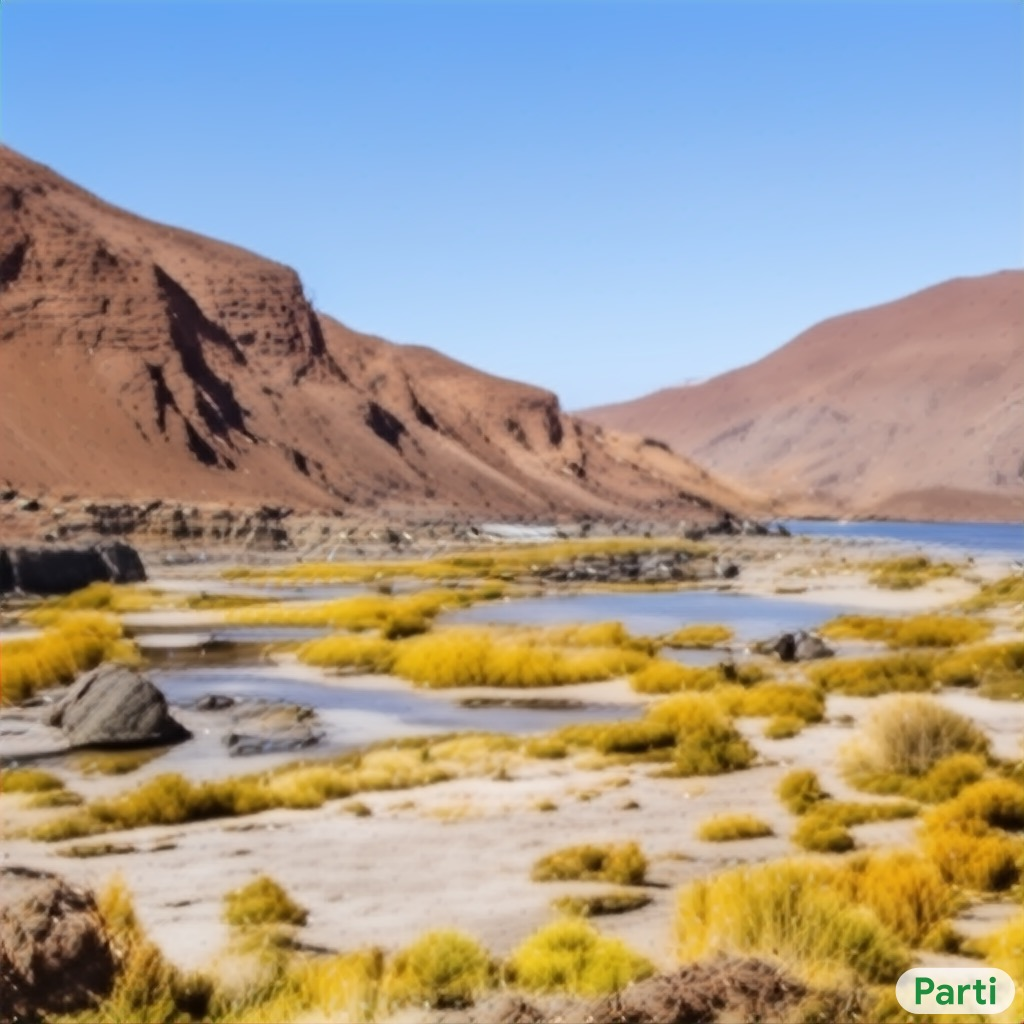
\includegraphics[width=0.19\textwidth]{figures/enc_pretrain/enc_pretrain_1_1.jpg} &
        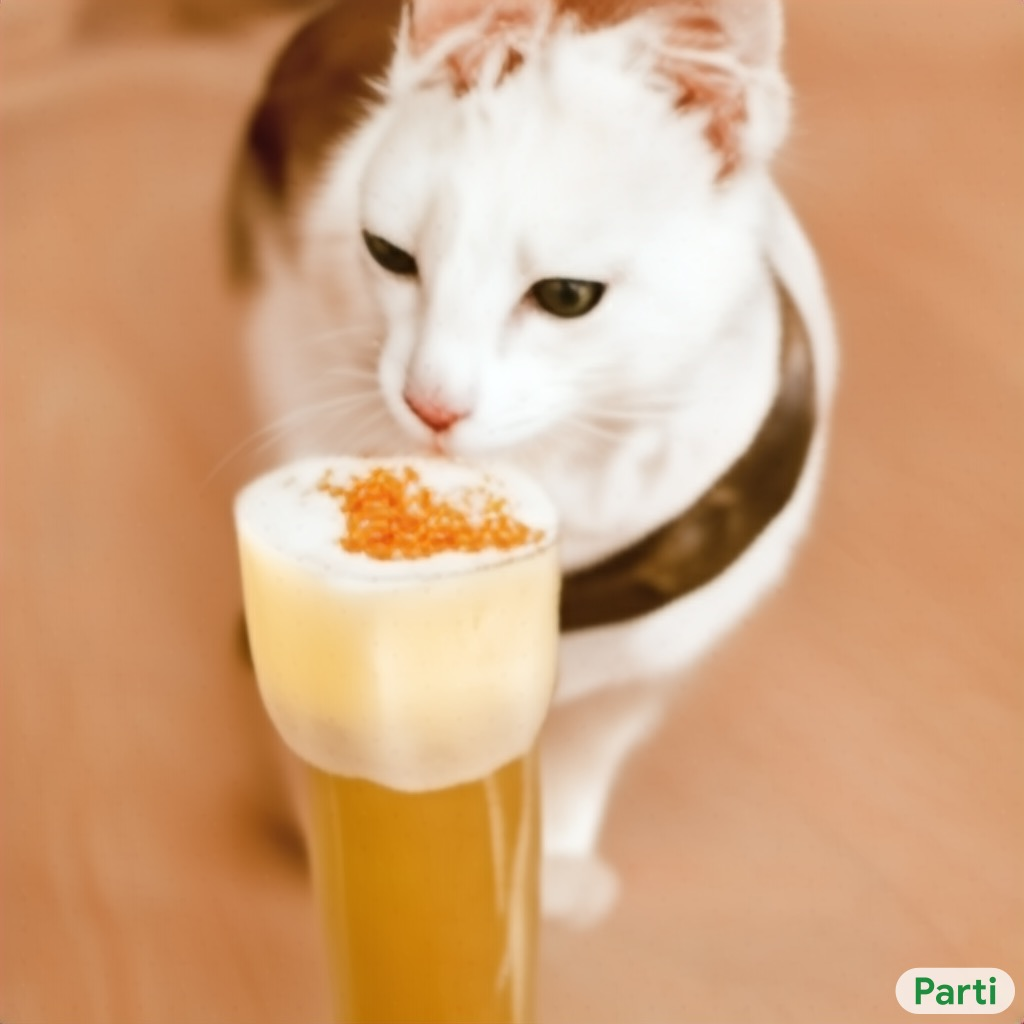
\includegraphics[width=0.19\textwidth]{figures/enc_pretrain/enc_pretrain_2_1.jpg} &
        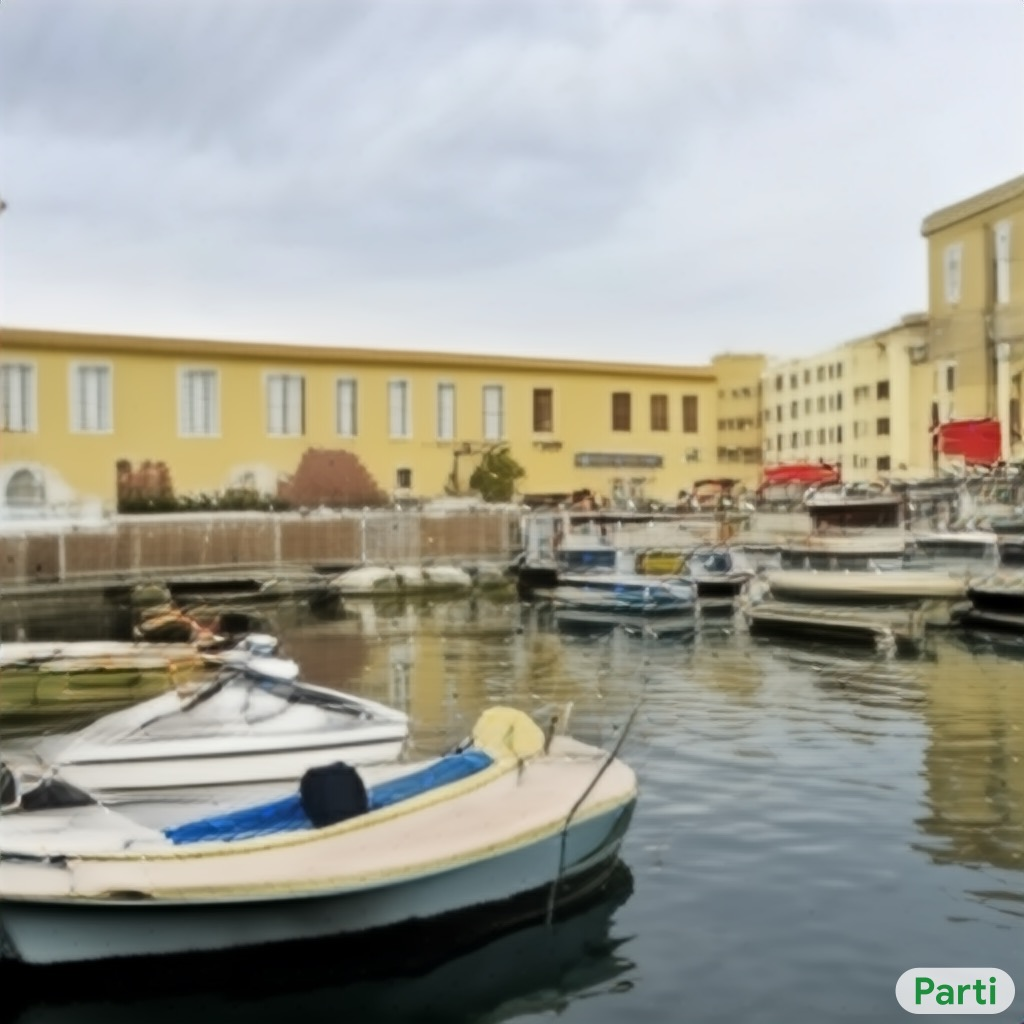
\includegraphics[width=0.19\textwidth]{figures/enc_pretrain/enc_pretrain_6_1.jpg} \\

        & \scriptsize \makecell{``a green clock in \\ the shape of a pentagon.''} 
        & \scriptsize \makecell{``a winding river \\ crosses the atacama desert.''}
        & \scriptsize \makecell{``a cat drinking \\ a pint of beer.''}          
        & \scriptsize \makecell{``a group of boats in \\ a harbor docked next to \\ a yellow building.''} \\
    \end{tabular}                                                                   
    \caption{Ablation of text encoder pretraining. In some of the prompts, we observe text-pretrained model outperforms non-pretrained encoders as examples shown above. However on average, we observe \textit{no significant} quality improvement by warming-up text encoder. Both models are with 3B parameters trained on the same mixture of datasets for ablation.}
    \label{figs:enc_pretrain}
\end{figure}